\section{Implementando una solución}

Para implementar alguna solución exacta del problema dado lo probado en la sección anterior, es decir, la pertenencia del problema a conjunto NP-completo habrá que diseñar algún algoritmo mediante la técnica de backtracking que pruebe todas las combinaciones existentes usando los conjuntos de subconjuntos. También se puede plantear alguna solución por programación lineal entera que resuelva el problema

\subsection{Backtracking}

Para construir una solución con una estrategia backtracking habrá que generar todas las posibles combinaciones entre los elementos pertenecientes a los conjuntos de subconjuntos. 

Para que sea una solución por backtracking y no por fuerza bruta (probar absolutamente todas las combinaciones) habrá que diseñar casos de poda, en otras palabras, realizar eliminaciones de posibles soluciones invalidas 

\subsubsection{Casos de poda}

Los casos de poda son esenciales para disminuir la duración en los tiempos de ejecución a la hora de buscar una solución al problema. En el caso particular de este problema, se habla sobre: 

\begin{itemize}
    \item \textbf{solución candidata}: que puede ser solución o no \\
    \item \textbf{solución encontrada}: un candidato a solución que esta validada como solución, pero puede no ser la mínima \\
    \item \textbf{solución mínima}: la solución más pequeña \\
\end{itemize}

Por lo tanto los casos de poda se determina de la siguiente manera: 

\begin{itemize}
    \item No se considera la secuencia si el candidato a solución es más grande que la solución anteriormente encontrada \\
    \item Si un subconjunto $i$ se encuentra incluido no se lo considera \\
    \item No se repite el uso de elementos entre subconjuntos en la solución encontrada \\
\end{itemize}

\subsubsection{Implementación}  
\begin{lstlisting}[language=Python, caption= solución por backtracking, label=python_code]
def has_a_player(subset, act_sol):
    for player in subset:
        if player in act_sol:
            return True
    return False

def search_for_min_hitting_set(subsets, a):
    return  _search_for_min_hitting_set(subsets, set(), set(), 0, set())

def _search_for_min_hitting_set(subsets: list, best_sol: set, act_sol: set, act_sub: int, used_players: set): 

    if len(best_sol) > 0 and len(act_sol) > len(best_sol): 
        return best_sol

    if act_sub == len(subsets) - 1 and (len(best_sol) == 0 or len(act_sol) < len(best_sol)) and is_solution(act_sol, subsets):
        best_sol = act_sol.copy()
        return best_sol
    
    if act_sub > len(subsets) - 1: 
        return best_sol

    if has_a_player(subsets[act_sub], act_sol):
        return _search_for_min_hitting_set(subsets, best_sol, act_sol, act_sub + 1, used_players)
    
    selected_players = set()

    for player in subsets[act_sub]:
        if player in used_players: 
            continue
        act_sol.add(player)
        selected_players.add(player)
        used_players.add(player)
        best_sol = _search_for_min_hitting_set(subsets, best_sol, act_sol, act_sub + 1, used_players)
        act_sol.remove(player)

    used_players.difference_update(selected_players)
    return best_sol
\end{lstlisting}

\subsubsection{Análisis de la complejidad}

Si bien es cierto que los casos de poda reducen el tiempo de ejecución del algoritmo no determinan una reducción teórica sobre el tiempo, es simplemente una manera de acelerar la apreciación experimental de conseguir una respuesta al problema. Por lo tanto la complejidad algorítmica del problema viene determinada por todas las combinaciones existentes en el problema, esto es entonces considerar todas las posibilidades sobre la pertenencia de un elemento del conjunto $b_{i_n}$, lo cual también puede ser visto como todas las combinaciones posibles sobre la pertenencia de los elementos del conjunto $C$

Por lo tanto:

$$
    T(n) = 2^n \text{ Siendo n = $|C|$}
$$


Es facíl, observar que una solución trivial al problema Hitting Set esta dada por todos los elementos del conjunto $C$

\subsection{ Programación lineal entera}

\subsubsection{Diseñando la solución por programación lineal}

Para generar una solución al Hitting Set problem mediante programación lineal entera se deben construir ecuaciones que modelen matemáticamente el problema. En un principio, el objetivo del problema es encontrar el mínimo de elementos de $C$ los cuales estén presentes en todos los conjuntos, por lo que, surge la primera ecuación: 
$$
\min \left( \sum_{i \in C} C_{i} \right)
$$
Con lo cual se construye la función objetivo del problema, evidentemente esta ecuación por si sola no es suficiente puesto que no considera el conjunto de subconjuntos  $B = B_1, B_2, ... B_m$ ($B_i \subseteq A \forall i$), faltaría entonces, exigir la pertenencia de al menos un elemento de cada subconjunto. Por lo que, surge la segunda y ultima ecuación necesaria para plantear el modelo:

$$
\sum_{b_j \in B_i} b_j \geq 1 \ \ \forall B_i \in B 
$$

También cabe aclarar que 

$$
b_j \in \{0, 1\}
$$

\subsubsection{Implementación}

Para construir una implementación con programación lineal entera se recurre a la librería \textbf{pulp} de python y se plantean las ecuaciones tal cual han sido descritas: 

\begin{lstlisting}[language=Python, caption= solución por programación líneal, label=python_code]
def search_hs_linealp(subsets, set):
    dict_variables = {elem: pulp.LpVariable(f"{elem}", cat="Binary") for elem in set}

    problem = pulp.LpProblem("hitting_set_problem", pulp.LpMinimize)
    problem += pulp.lpSum(dict_variables[elem] for elem in set)
    for subset in subsets:
        problem += pulp.lpSum(dict_variables[elem] for elem in subset) >= 1
    
    pulp.LpSolverDefault.msg = 0
    problem.solve()
    
    hitting_set_solution = {var.name for var in dict_variables.values() if pulp.value(var) == 1}
    return hitting_set_solution

\end{lstlisting}

Cabe destacar que esta solución requiere el paso previo de la reconstrucción del conjunto $C$, lo cual se realiza fácilmente usando diccionarios 

\subsubsection{Análisis de la complejidad}

La programación lineal entera esta clasificada también como un problema NP-Completo (\href{https://en.wikipedia.org/wiki/Integer_programming}{véase la referencia}) y analizando un poco más las ecuaciones planteadas llegamos a que simplemente es una formulación de las posibles soluciones también consideradas en la resolución del problema mediante backtracking, por lo que tenemos que la complejidad temporal del algoritmo es también: 

\begin{samepage}
\[
T(n) = 2^n \quad \text{Siendo } n = |C|
\]
\end{samepage}

\section{Gráficas}

A continuación se introducen una serie de gráficas con la intención de observar el comportamiento de las dos implementaciones que consiguen el mínimo global al Hitting Set Problem

Se generaron datos aleatorios mediante la biblioteca Faker que permite la generación de nombres. Se generaron doscientos nombres aleatorios y a partir de allí se generan conjuntos de subconjuntos para todos los m $\in \ (1, 200)$ de manera que se puedan apreciar bien las complejidades del algoritmo 

\subsection{Tiempos de la resolución por backtracking }

\begin{figure}[H]
    \centering
    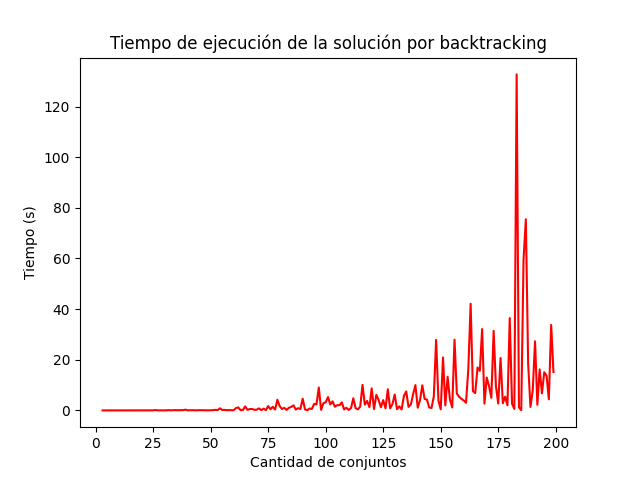
\includegraphics[width=0.6\textwidth]{graficos/backtracking.png}
\end{figure}

En la gráfica anterior se observan los tiempos de ejecución para la implementación usando backtracking, es importante destacar la gran variabilidad entre los tiempos de ejecución existentes entre los conjuntos. Esto se debe a la variabilidad que existe entre los conjuntos con los cuales se va probando en cada paso el algoritmo 

\subsection{Tiempos de ejecución por Programación Entera}

\begin{figure}[H]
    \centering
    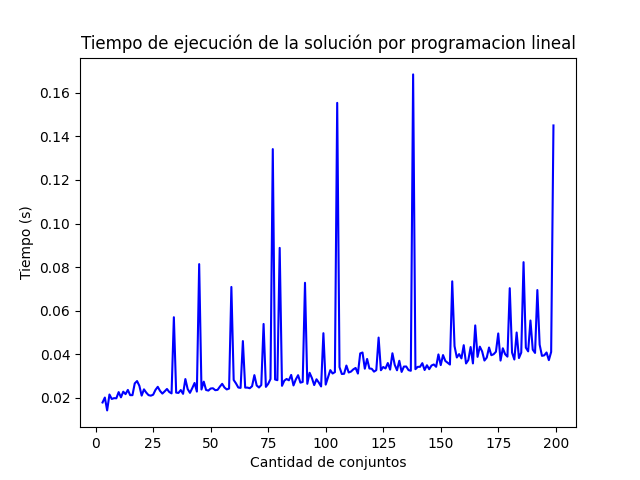
\includegraphics[width=0.6\textwidth]{graficos/integerp.png}
\end{figure}

Por otro lado los tiempos de ejecución para la solución por programación lineal entera son más pequeños en comparación a la solución por backtracking. Debido al uso de la biblioteca \textbf{pulp} se estima que dicha resolución cuenta con optimizaciones ocultas al desarrollador y por lo tanto pareciera que la tendencia temporal tiende a ser algo lineal 

\subsection{Comparación entre ambos métodos}

Finalmente se grafican sobre una misma escala ambos métodos y se aprecia la amplia diferencia entre ambos

\begin{figure}[H]
    \centering
    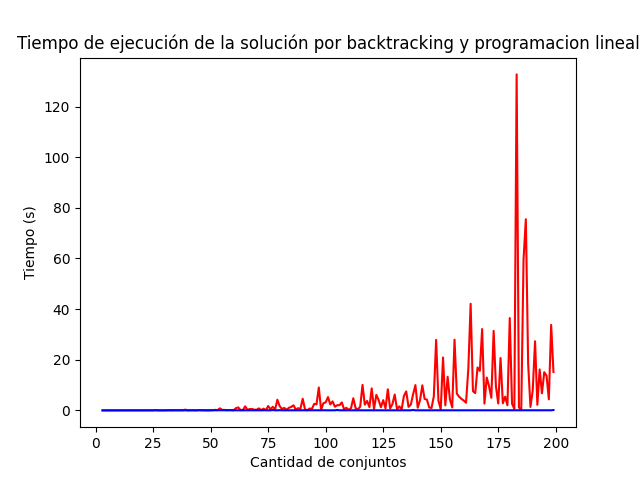
\includegraphics[width=0.6\textwidth]{graficos/ilpvsbt.png}
\end{figure}

\section{Estimación contra cota teórica}

\subsection{Backtracking acotado por curva teórica}

Se genero una gráfica con una curva teórica exponencial, con lo cual se puede apreciar que la implementación por backtracking se comporta efectivamente de manera exponencial al conjunto de entrada 

\begin{figure}[H]
    \centering
    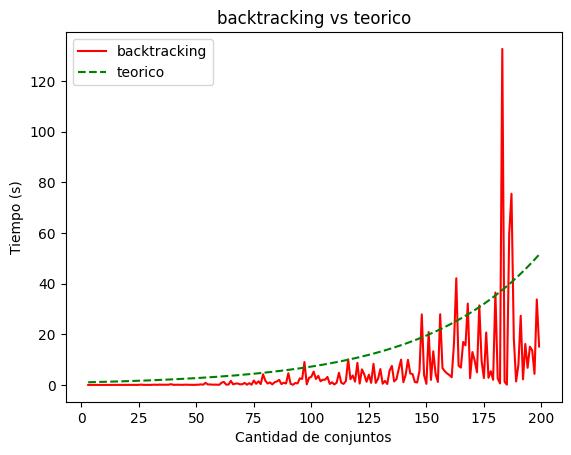
\includegraphics[width=0.6\textwidth]{graficos/backvsteorico.png}
\end{figure}
